% !TEX program = xelatex
\documentclass[a4paper, 12pt]{article}

\usepackage[UTF8]{ctex}     % 支持中文
\usepackage{geometry}       % 页面边距设置
\usepackage{graphicx}       % 插入图片
\usepackage{booktabs}       % 三线表
\usepackage{float}          % 固定图片和表格位置 [H]
\usepackage{subcaption}     % 支持子图排版 (用于5张热力图)
\usepackage{hyperref}       % 超链接
\usepackage{tabularx}       % 自动调整宽度的表格

% 设置页面边距
\geometry{left=2.5cm, right=2.5cm, top=2.5cm, bottom=2.5cm}

% 取消段落首行缩进，增加段间距（可选，使排版更现代）
\setlength{\parindent}{2em}
\setlength{\parskip}{0.5em}

\begin{document}

% ==================== 1. 封面 ====================
\begin{titlepage}
    \centering
    \vspace*{3cm}
    
    {\Huge \bfseries 2026春季人工智能导论\par}
    \vspace{1cm}
    {\LARGE \bfseries 项目中期报告\par}
    \vspace{1.5cm}
    
    {\Large \bfseries 基于 ViT 与 CNN 在 CIFAR-10 上的 \\ 图像分类性能对比研究\par}
    \vspace{3cm}
    
    {\large \bfseries 团队成员与任务分工}\par
    \vspace{0.5cm}
    
    \begin{table}[H]
    \centering
    \renewcommand{\arraystretch}{1.5}
    % 使用 tabularx，总宽度设为 0.9\textwidth，第二列使用 X 格式以自动换行
    \begin{tabularx}{0.9\textwidth}{c|X}
        \toprule
        \textbf{姓名} & \textbf{主要负责模块与分工内容} \\
        \midrule
        黄泽皓 & 主导数据与训练 Pipeline。负责数据加载、预处理与增强，编写模型训练循环及指标评测逻辑。 \\
        \hline
        张一 & 主导模型核心实现。负责基于 PyTorch 从零搭建 Vision Transformer 的核心组件，构建对比基线 CNN 模型。 \\
        \hline
        刘梵佑 & 主导实验调度、可视化与报告撰写。负责完成 Attention Map 生成及图表整理；相关可视化源码将在后续仓库版本中补充同步。 \\
        \bottomrule
    \end{tabularx}
\end{table}
    
    \vfill
    %{\large 学校：复旦大学\par}
    %{\large 提交日期：\today\par}
\end{titlepage}

\newpage

% ==================== 2. 任务与数据 ====================
\section{任务与数据说明}

\subsection{问题定义}
本项目旨在完成 CIFAR-10 数据集的图像分类任务，并横向对比经典卷积神经网络（CNN）与视觉变换器（Vision Transformer, ViT）在不同数据量级下的性能表现。为了全面评估模型的表现，我们选定了以下三个核心评价指标：
\begin{itemize}
    \item \textbf{分类准确率 (Accuracy)}：衡量模型在测试集上预测正确的样本比例。
    \item \textbf{宏观 F1 分数 (Macro-F1)}：综合考量模型在 10 个类别上的精确率与召回率表现，避免类别不平衡带来的评估偏差。
    \item \textbf{训练效率 (Time/epoch)}：记录单轮训练（Epoch）所需的时间，用于评估模型的计算开销与工程可行性。
\end{itemize}

\subsection{数据说明与预处理}
实验采用 64$\times$64 高分辨率版本的 CIFAR-10 数据集，包含 10 个常见物体类别，总计划分为 50,000 张训练集与 10,000 张测试集。在数据预处理与增强阶段，我们执行了以下操作：
\begin{enumerate}
    \item \textbf{归一化 (Normalization)}：使用标准均值 \texttt{[0.4914, 0.4822, 0.4465]} 和标准差 \texttt{[0.2023, 0.1994, 0.2010]} 进行数据标准化。
    \item \textbf{数据增强 (Data Augmentation)}：仅针对训练集启用了随机水平翻转（RandomHorizontalFlip），以提升模型的泛化能力。
    \item \textbf{子集采样 (Subset Sampling)}：针对后续的小数据退化实验，我们在 \texttt{dataset.py} 中构建了基于 \texttt{numpy.random.permutation} 的随机子集采样逻辑，可支持按照 20\% 与 10\% 比例进行无偏采样。
\end{enumerate}

% ==================== 3. 模型设计 ====================
\section{模型设计}
为了实现公平的横向对比，我们在设计上严格控制了 CNN 与 ViT 的参数量级（Params），确保两者在相近的模型容量下进行学习能力的对标。

\subsection{卷积神经网络 (CNN) 架构}
基线 CNN 模型自行设计了一个 4 层深度的卷积神经网络架构，其结构特点如下：
\begin{itemize}
    \item \textbf{通道递增}：网络特征通道数随深度依次翻倍（64 $\rightarrow$ 128 $\rightarrow$ 256 $\rightarrow$ 512）。
    \item \textbf{卷积块设计}：每个特征提取阶段采用标准的 \texttt{Conv-BN-ReLU-Conv-BN-ReLU-MaxPool-Dropout} 现代特征提取范式。
    \item \textbf{分类头}：摒弃了传统大参数量的全连接层展平方式，采用全局平均池化层（Global Average Pooling, GAP），将特征图直接压缩至一维向量，随后送入带有 Dropout 的两层 MLP 分类器，有效减少了参数冗余。
\end{itemize}

\subsection{视觉变换器 (ViT) 架构}
ViT 模型完全基于 PyTorch 从零手写搭建，其核心超参数配置如表~\ref{tab:vit_hyperparams} 所示。模型采用了 Pre-LN 结构的 Transformer Block，引入了随机深度（Stochastic Depth / DropPath）以增强网络深层训练的稳定性，并通过可学习的 CLS Token 汇总全局特征进行分类。
实验训练版本中，\texttt{config.py} 已作为集中式超参数入口接入训练流程，用于统一管理层数、heads、patch size、embed dim、batch size 等关键配置；当前中期仓库快照中的训练脚本尚未完全同步该版本，后续将补齐代码版本一致性。

% 超参表格
\begin{table}[H]
    \centering
    \caption{Vision Transformer (ViT) 核心超参数配置表}
    \label{tab:vit_hyperparams}
    \renewcommand{\arraystretch}{1.2}
    \begin{tabular}{lc|lc}
        \toprule
        \textbf{超参数名称} & \textbf{设定值} & \textbf{超参数名称} & \textbf{设定值} \\
        \midrule
        输入图像尺寸 (img\_size) & $64 \times 64$ & 注意力头数 (num\_heads) & 8 \\
        分块尺寸 (patch\_size) & $8 \times 8$   & MLP 扩展比例 (mlp\_ratio) & 4.0 \\
        Patch 数量 (num\_patches)& 64             & Dropout 概率 (dropout) & 0.1 \\
        嵌入维度 (embed\_dim)    & 256            & DropPath 概率 & 0.1 \\
        Transformer 层数 (depth)& 6              & 分类类别数 (num\_classes) & 10 \\
        \bottomrule
    \end{tabular}
\end{table}

% ViT 架构图占位符
\begin{figure}[H]
    \centering
    % 请将 vit_architecture.png 替换为您准备好的ViT架构图文件名
    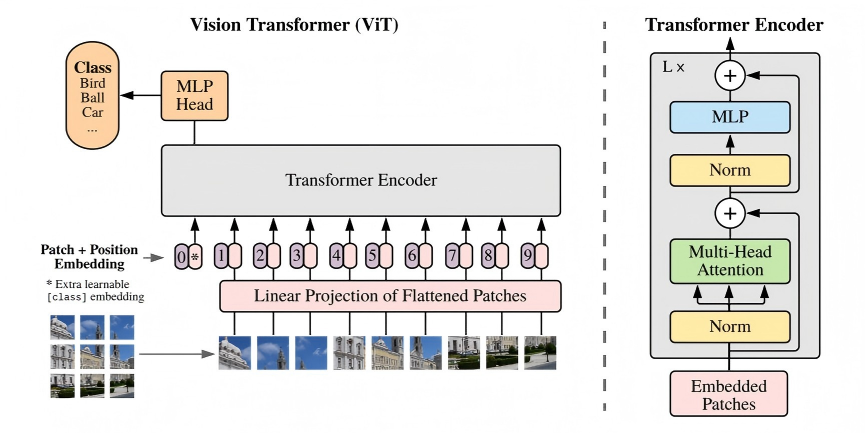
\includegraphics[width=0.6\textwidth]{vit_architecture.png}
    
    % 下面是一个纯文本的占位框，实际编译时请使用上一行的 \includegraphics
    %\framebox(400, 150){\Large [请在此处插入 ViT 架构图：vit\_architecture.png]}
    \caption{Vision Transformer (ViT) 整体架构示意图}
    \label{fig:vit_arch}
\end{figure}


% ==================== 4. 已有实验结果 ====================
\section{实验结果与分析}

\subsection{多维度性能指标汇总}
我们完成了针对 CNN 与 ViT 在三档数据比例（10\%、20\%、100\%）下的完整训练测试。实验结果如表 \ref{tab:all_results} 所示，展现了两种架构在不同数据规模下的适应性差异。

\begin{table}[H]
    \centering
    \caption{CNN 与 ViT 在不同数据比例下的性能对比汇总}
    \label{tab:all_results}
    \renewcommand{\arraystretch}{1.2}
    \begin{tabularx}{\textwidth}{l|c|ccc}
        \toprule
        \textbf{模型架构} & \textbf{数据比例} & \textbf{测试准确率 (Acc)} & \textbf{Macro-F1} & \textbf{单轮耗时 (s)} \\
        \midrule
        \textbf{CNN} & 10\%  & 70.95\% & 0.7090 & 18.42 \\
        (自定义 4 层 CNN)  & 20\%  & 79.89\% & 0.7986 & 24.53 \\
                     & 100\% & 90.41\% & 0.9038 & 61.30 \\
        \hline
        \textbf{ViT} & 10\%  & 56.37\% & 0.5600 & 28.05 \\
        (手搓版)     & 20\%  & 63.31\% & 0.6300 & 41.95 \\
                     & 100\% & 80.71\% & 0.8059 & 152.82 \\
        \bottomrule
    \end{tabularx}
\end{table}

从表 2 的结果可以清晰看出两种架构的特性差异。在 10\% 与 20\% 的极小数据场景下，CNN 凭借卷积核天然的平移不变性与局部感知（归纳偏置），达到了 70.95\% 与 79.89\% 的准确率；而同等数据量下，ViT 仅有 56.37\% 与 63.31\%，出现了严重的性能退化。这有力地证明了全局自注意力机制在缺乏足够数据驱动时，极难自发学到有用的图像空间结构。但随着数据量扩展至 100\%，ViT 的准确率获得了近 24 个百分点的巨大增幅（跃升至 80.71\%），展现出惊人的数据扩展潜力。

% ==================== 3.2 训练曲线对比分析 ====================
\subsection{训练曲线对比分析（数据效率实验）}

为深入探究 CNN 与 ViT 在不同数据规模下的收敛特性，我们生成了包含左右双子图的综合对比图（见图 \ref{fig:learning_curves}）。左侧子图展示了训练损失（Loss）的下降趋势，右侧子图展示了测试准确率（Accuracy）的演进过程。

通过颜色与线型的多维编码，图表清晰地呈现了实验规律：
\begin{itemize}
    \item \textbf{颜色编码（架构区别）}：蓝色系代表自定义 CNN，橙/红色系代表 ViT。
    \item \textbf{线型编码（数据比例）}：
    \begin{itemize}
        \item \textbf{10\% 数据量}：浅色 + 点虚线 (\texttt{:})
        \item \textbf{20\% 数据量}：中等色 + 虚线 (\texttt{--})
        \item \textbf{100\% 数据量}：深色加粗 + 实线 (\texttt{-})
    \end{itemize}
\end{itemize}

\begin{figure}[H]
    \centering
    % 请确保文件名与你保存的图片一致
    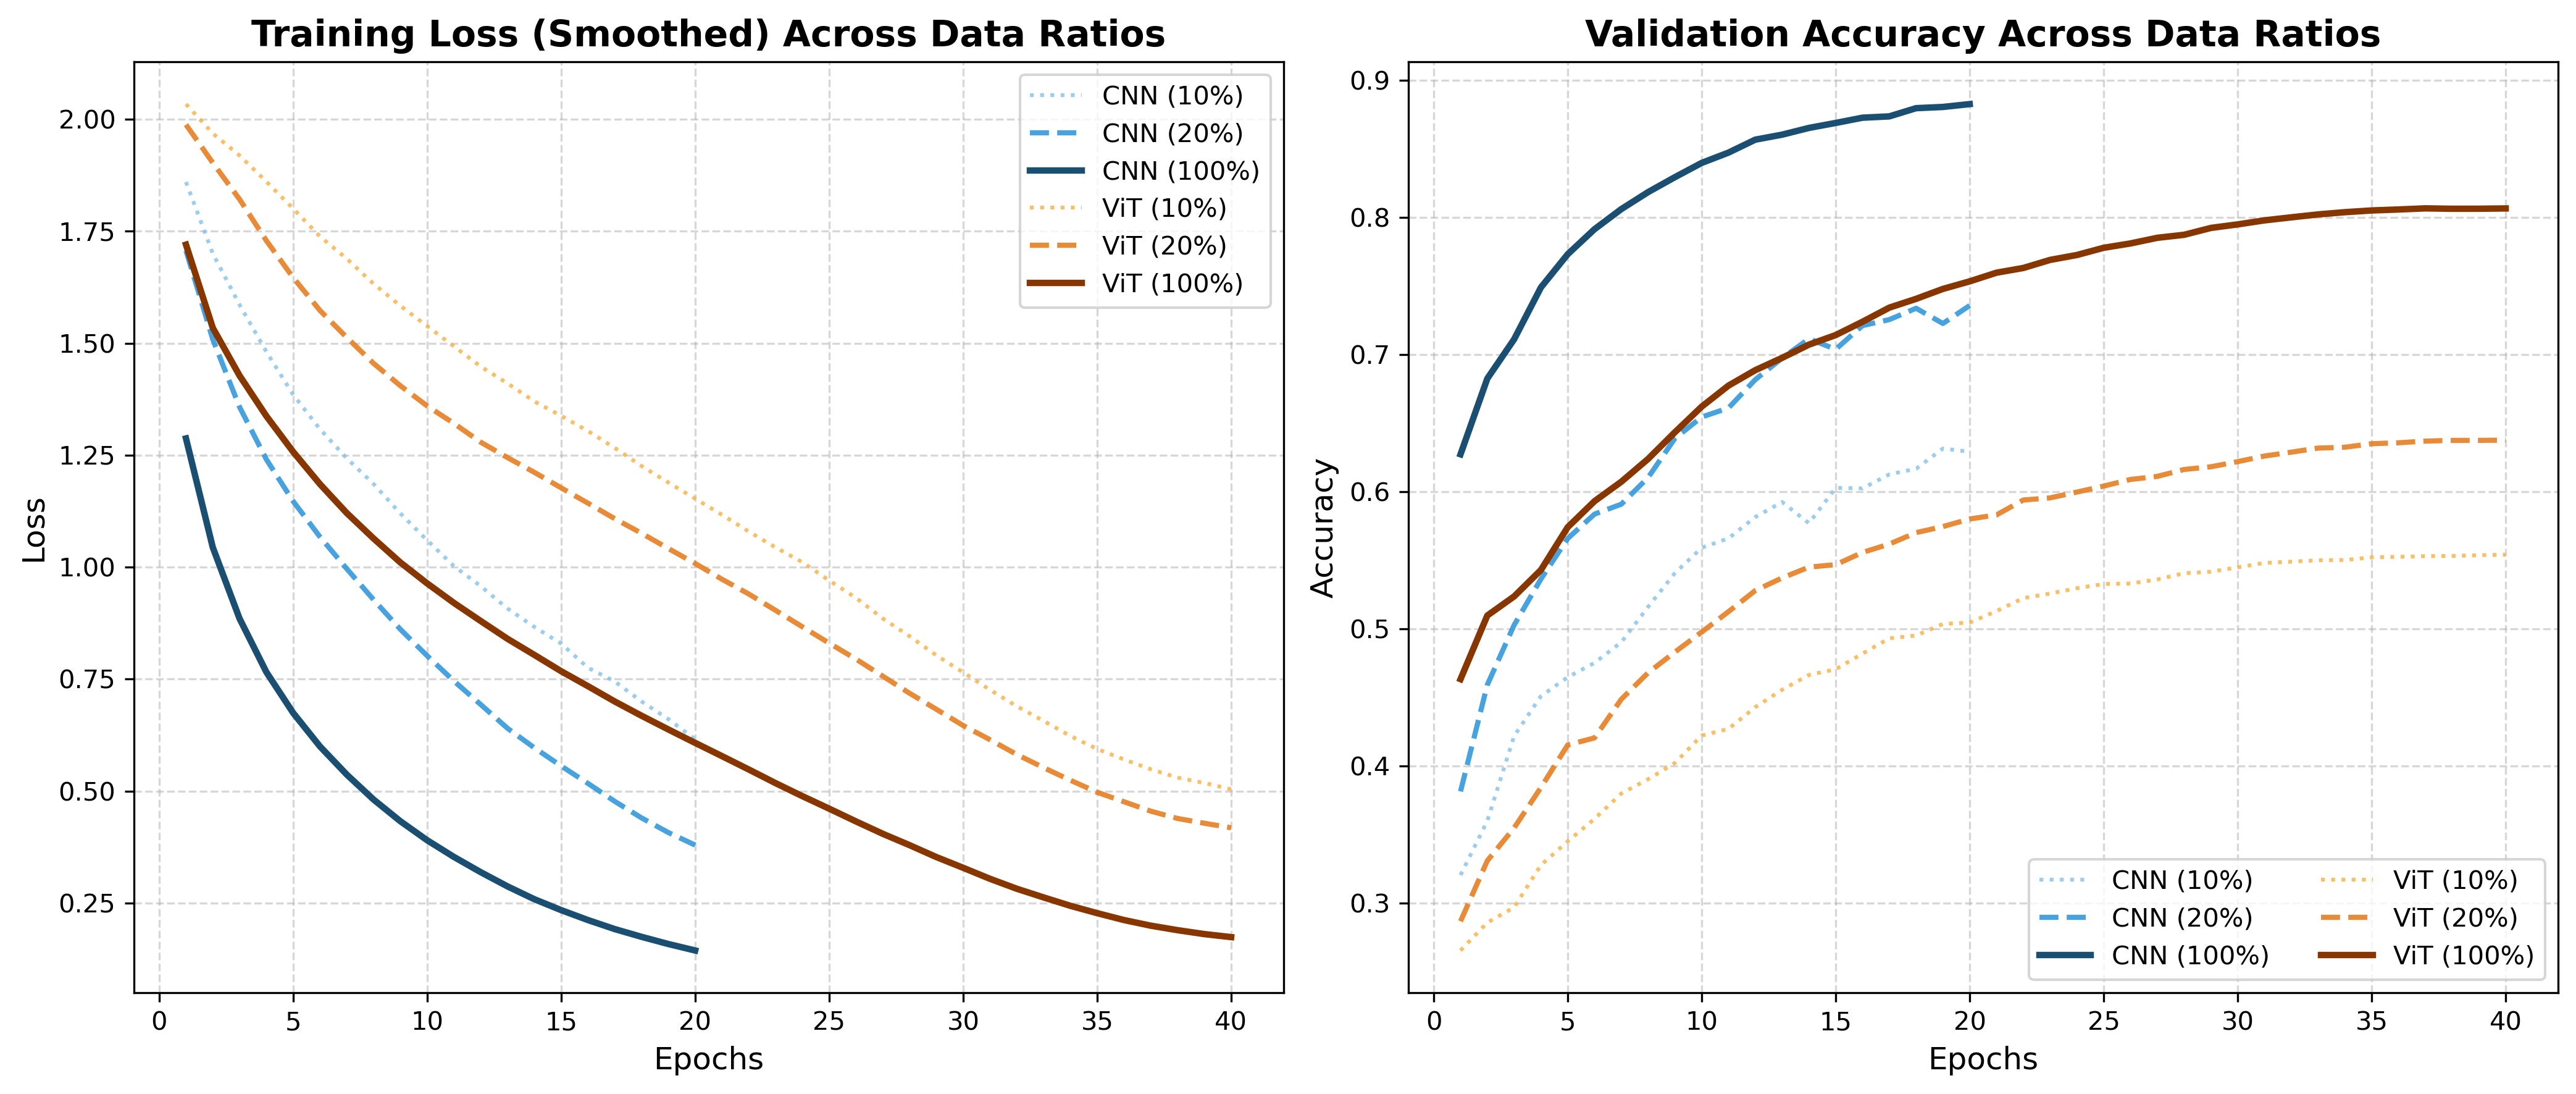
\includegraphics[width=0.95\textwidth]{learning_curve_all.png}
    
    % 占位框（出图后可删除此行）
    %\framebox(450, 220){\Large [请在此处插入双子图：cnn\_vit\_comparison\_dual.png]}
    
    \caption{CNN 与 ViT 在 0.1、0.2、1.0 三档数据比例下的训练曲线对比。左图：训练损失曲线；右图：测试集准确率曲线。}
    \label{fig:learning_curves}
\end{figure}

\subsubsection{结果分析：归纳偏置与 Scaling Law 的博弈}
根据表 \ref{tab:all_results} 的量化指标与图 \ref{fig:learning_curves} 的可视化曲线，我们可以得出以下关键发现：

\begin{enumerate}
    \item \textbf{CNN 的小数据稳健性}：在 10\% 数据（5,000 张）极度匮乏的情况下，CNN 依然能达到 70.95\% 的准确率，而 ViT 仅为 56.37\% 。这证明了卷积操作自带的局部平移不变性等“归纳偏置”在小样本学习中起到了决定性的先验辅助作用。
    \item \textbf{ViT 的高上限与 Scaling 性质}：随着数据比例从 0.1 提升至 1.0，ViT 的准确率从 56.37\% 巨幅提升至 80.71\% ，表现出比 CNN 更强的“数据饥渴”特性和性能天花板。
    \item \textbf{收敛稳定性}：观察 Loss 曲线可以发现，ViT 的曲线在训练初期波动较大，且对学习率（LR）及 Warmup 策略更为敏感；相比之下，CNN 的蓝色实线在各数据量下均表现出更快的下降速度与更平滑的收敛路径。
\end{enumerate}

\subsection{ViT 模型 Attention Map 可视化}
为探究 ViT 模型对图像特征的全局感知与捕捉能力，我们提取了 Transformer 编码器层的 Attention Weights，并针对验证集样本生成了热力图。图 3 展示了 6 个不同样本的注意力集中区域，红色/高亮部分代表分类 Token（CLS）在决策时主要聚焦的输入 Patch。
本次中期仓库中已保留生成后的 Attention Map 图像文件，但可视化负责队员尚未将对应生成脚本同步上传，因此当前仓库暂不包含该部分源码；后续版本将补充脚本以提升结果复现性。

\begin{figure}[H]
    \centering
    
    % ========== 第一排：并列 3 张图 ==========
    \begin{subfigure}{0.31\linewidth}
        \centering
        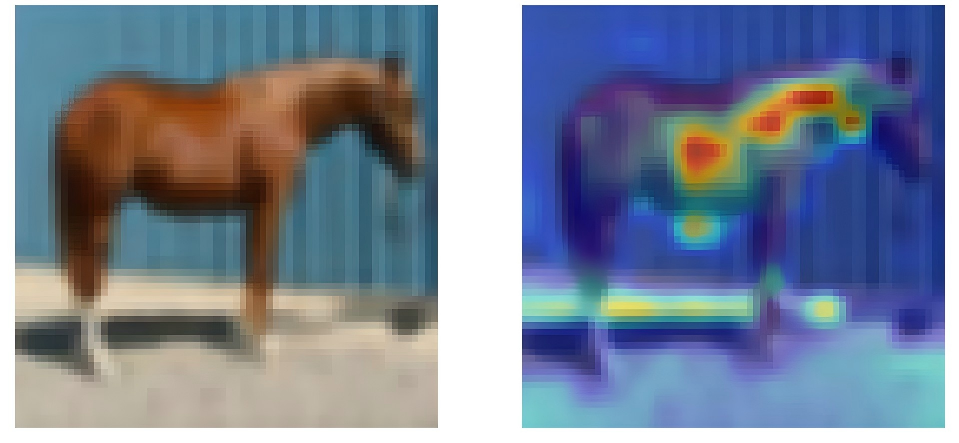
\includegraphics[width=\linewidth]{heatmap_1.png}
        %\framebox(120, 90){图 1}
    \end{subfigure}\hfill
    \begin{subfigure}{0.31\linewidth}
        \centering
        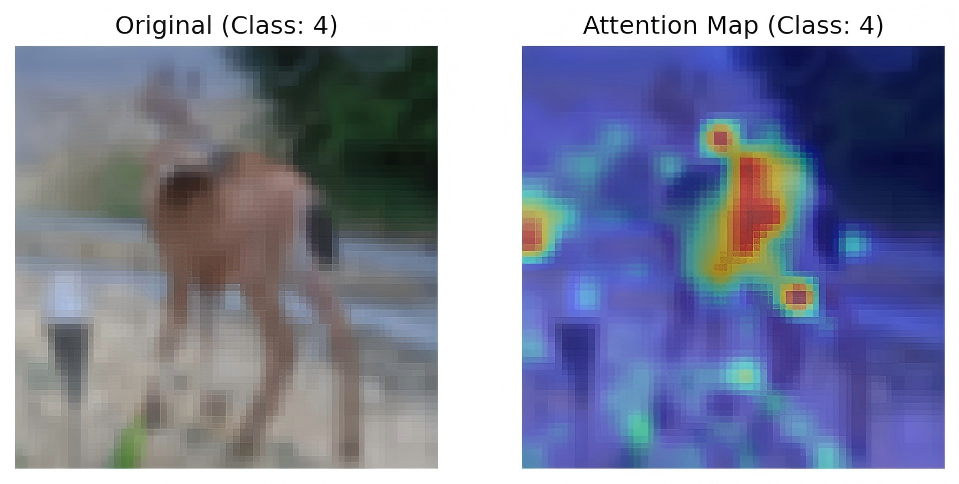
\includegraphics[width=\linewidth]{heatmap_2.png}
        %\framebox(120, 90){图 2}
    \end{subfigure}\hfill
    \begin{subfigure}{0.31\linewidth}
        \centering
        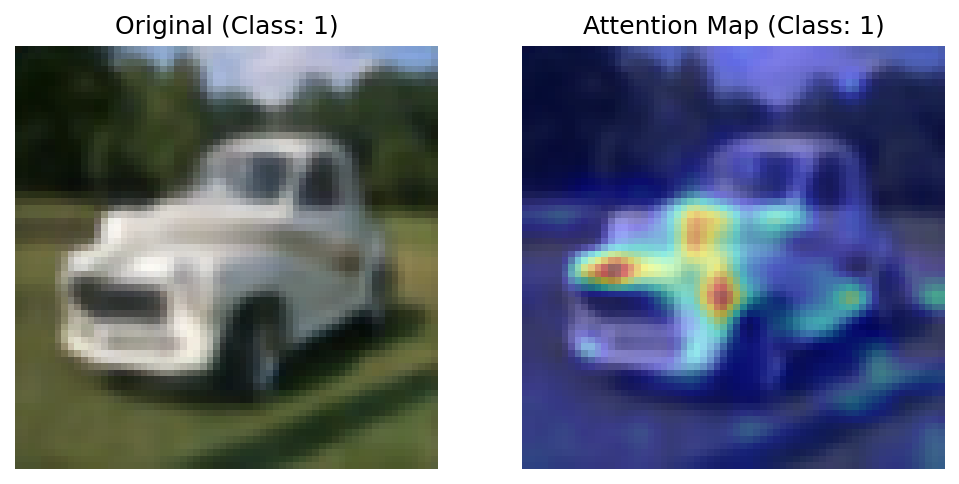
\includegraphics[width=\linewidth]{heatmap_3.png}
        %\framebox(120, 90){图 3}
    \end{subfigure}
    
    \vspace{1.5em} % 两排之间的垂直间距
    
    % ========== 第二排：并列 2 张图（居中） ==========
    \begin{subfigure}{0.31\linewidth}
        \centering
        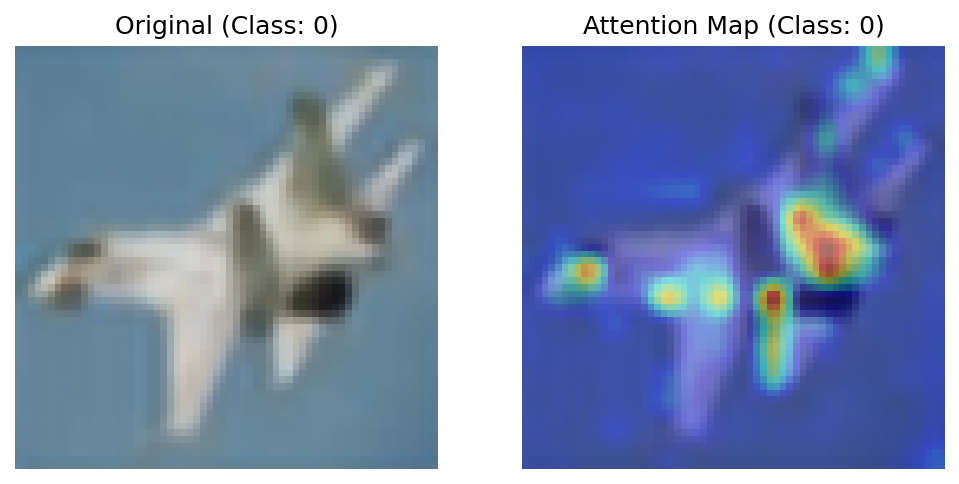
\includegraphics[width=\linewidth]{heatmap_4.png}
        %\framebox(120, 90){图 1}
    \end{subfigure}\hfill
    \begin{subfigure}{0.31\linewidth}
        \centering
        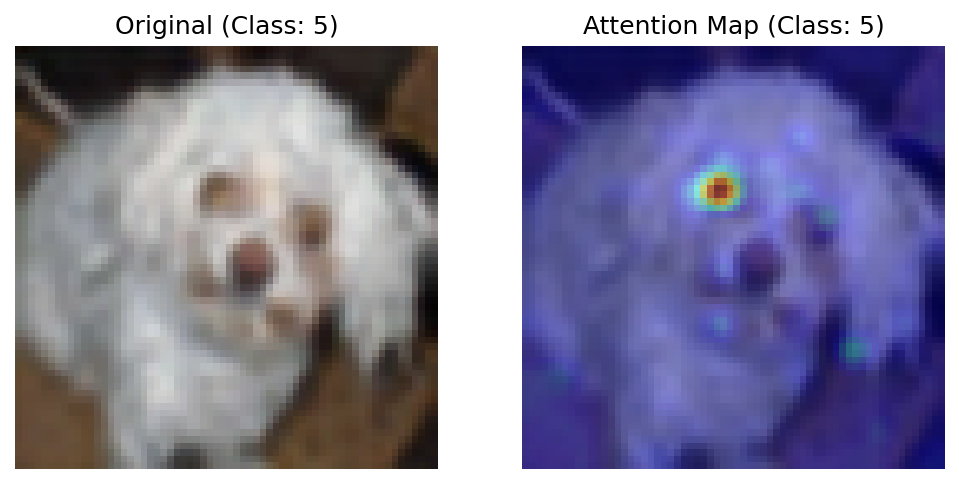
\includegraphics[width=\linewidth]{heatmap_5.png}
        %\framebox(120, 90){图 2}
    \end{subfigure}\hfill
    \begin{subfigure}{0.31\linewidth}
        \centering
        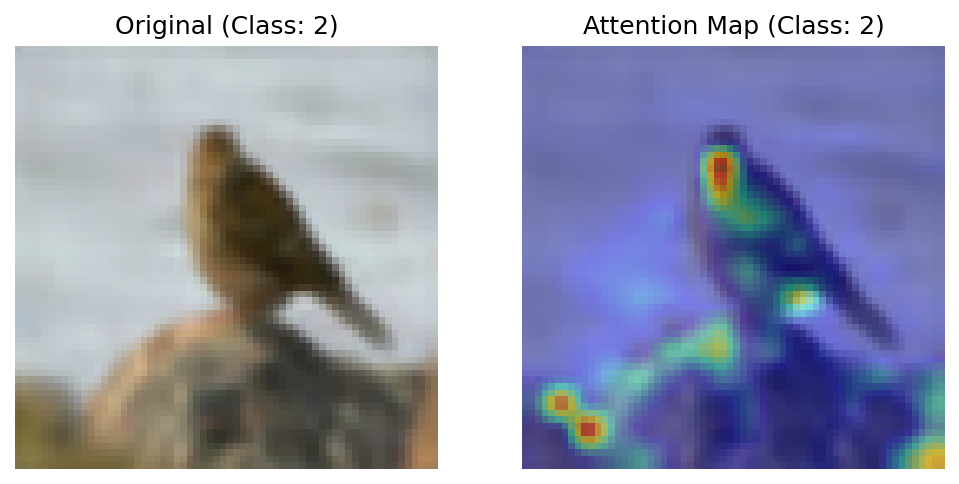
\includegraphics[width=\linewidth]{heatmap_6.png}
        %\framebox(120, 90){图 3}
    \end{subfigure}
    
    \caption{ViT 模型的 Attention Map 热力图可视化。高亮区域代表模型主要关注的特征区域。}
    \label{fig:heatmaps}
\end{figure}

\subsection{速度与精度权衡 (Speed-Accuracy Trade-off)}

为直观展示不同模型架构及数据规模下的计算开销与分类性能关系，我们绘制了速度-精度权衡散点图。不同实验设置（模型架构 $\times$ 数据量比例）将作为独立的数据点呈现，从而综合评估 ViT 与 CNN 的工程部署性价比。

\begin{figure}[H]
    \centering
    % 请在后续画出图表后，将 speed_accuracy_tradeoff.png 放入文件夹，并取消下一行的注释
    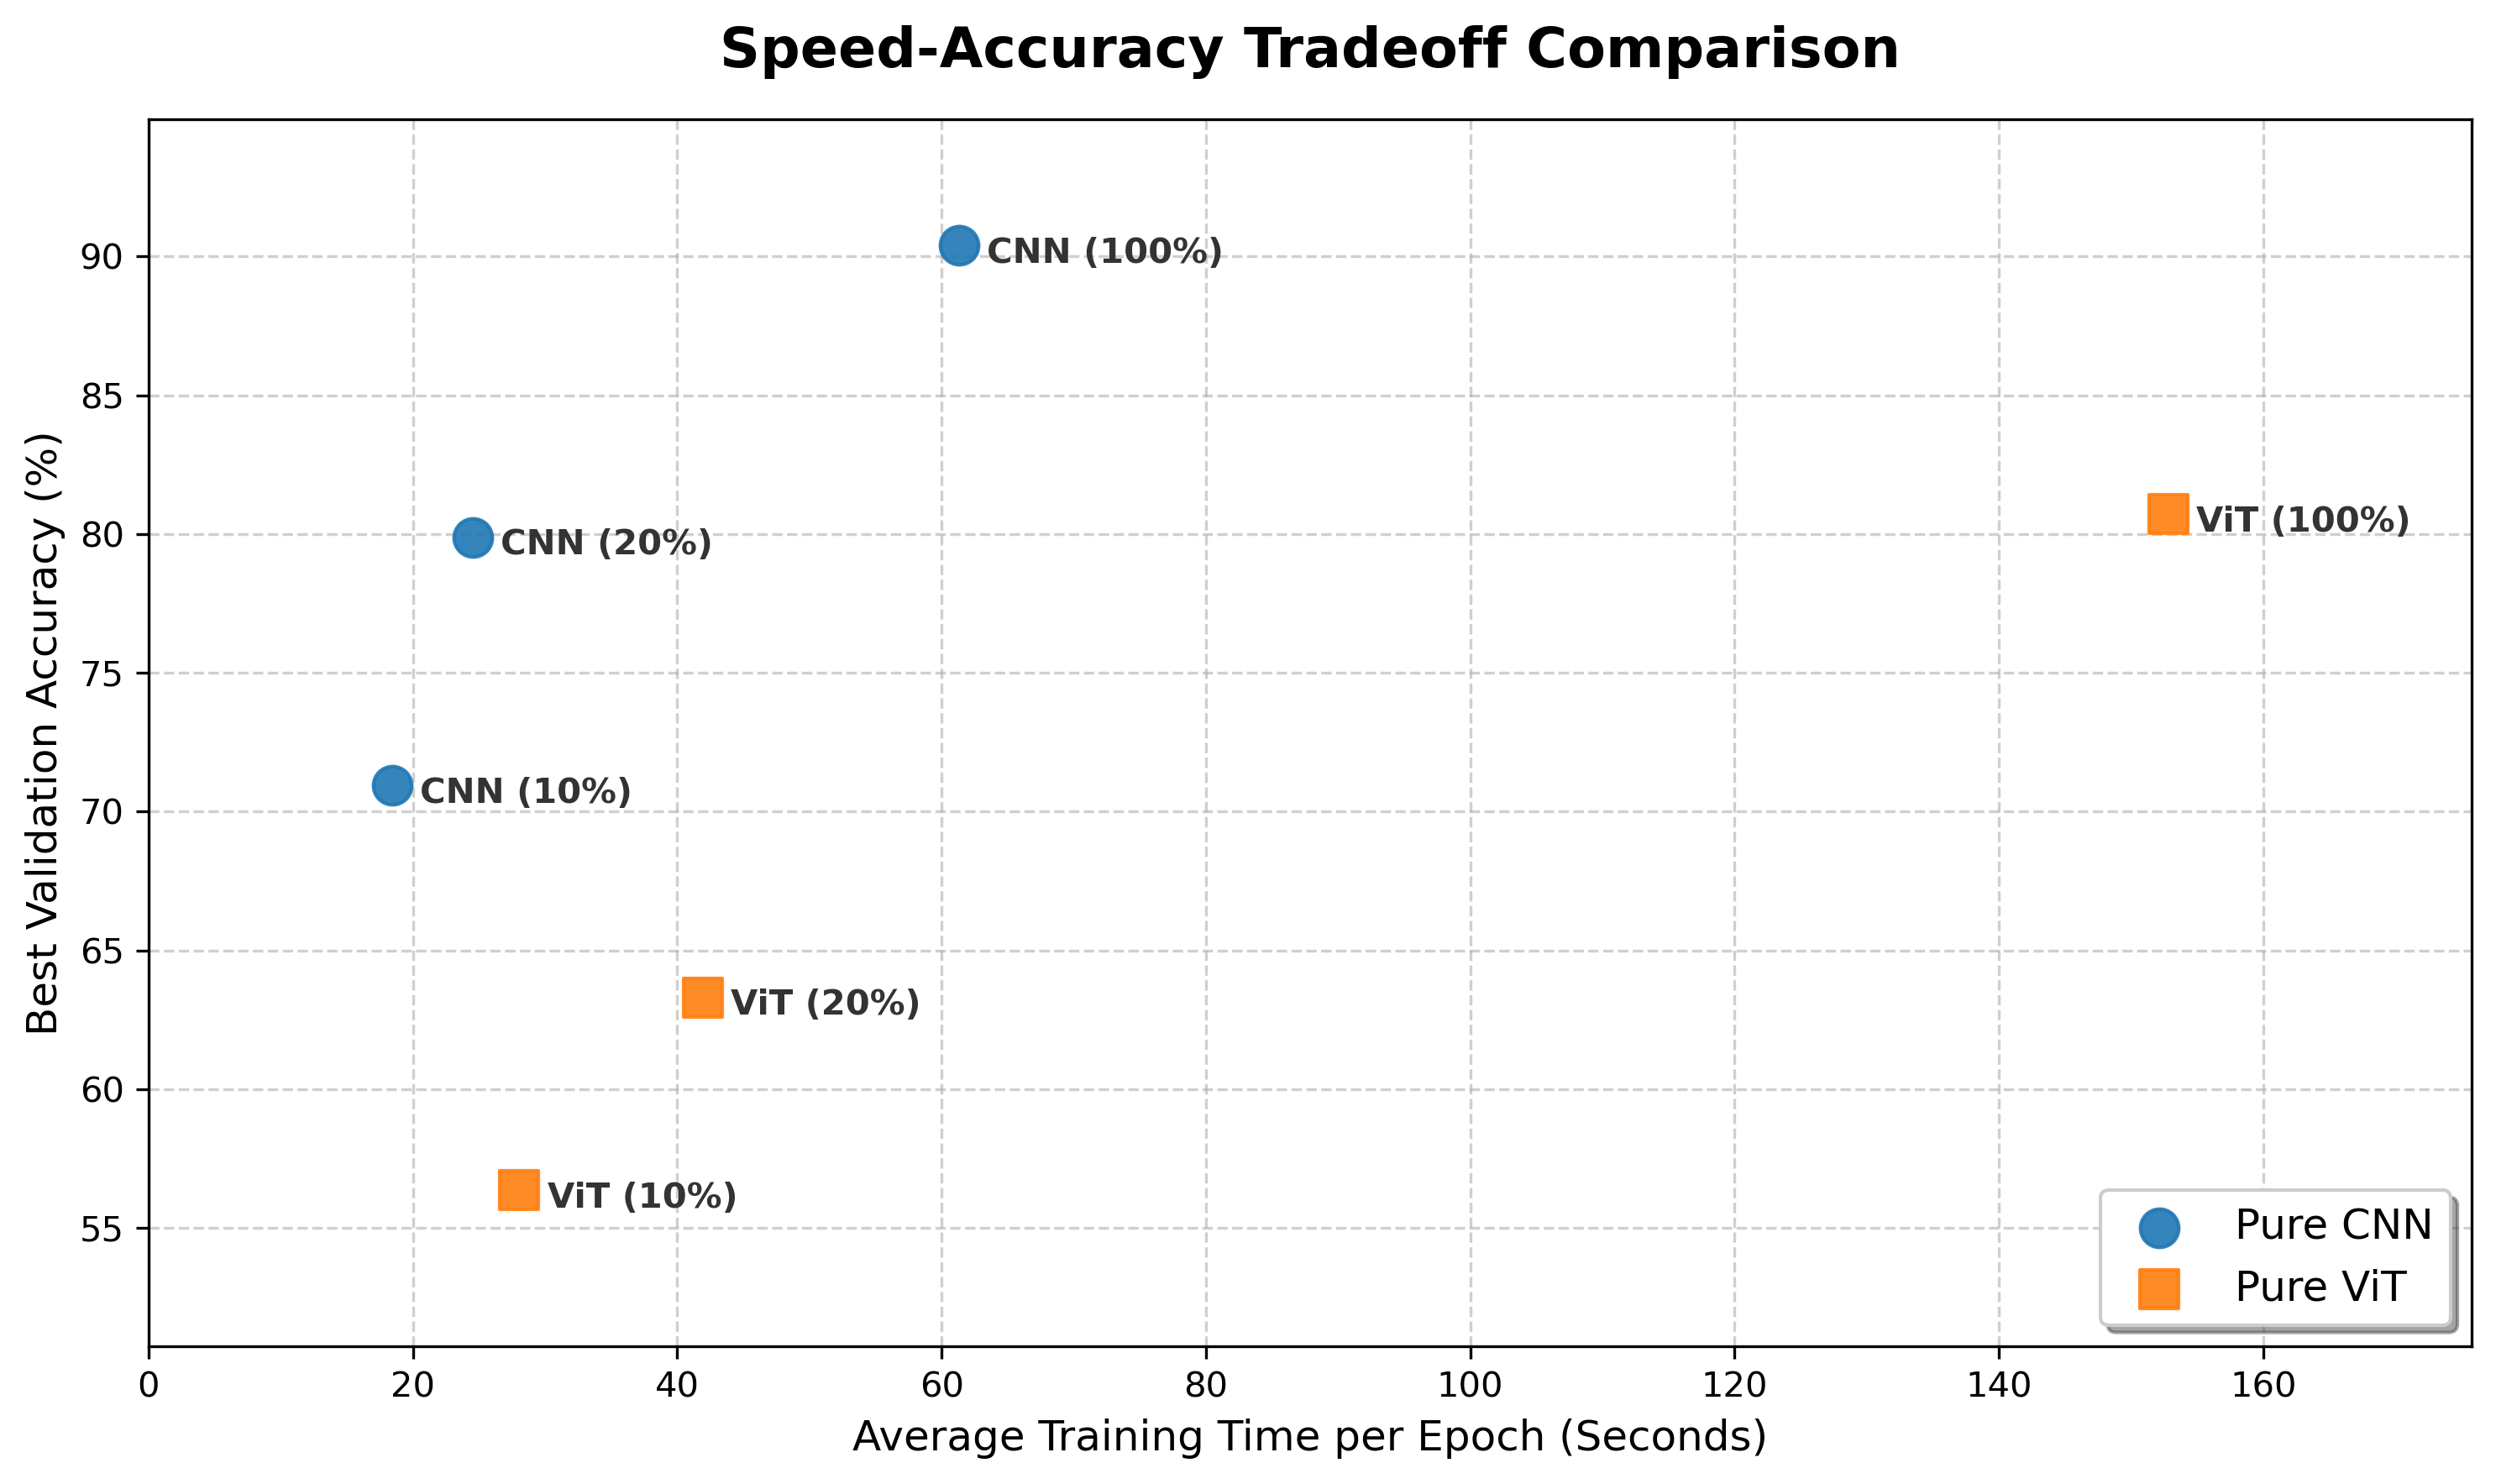
\includegraphics[width=0.75\textwidth]{speed_accuracy_tradeoff.png}
    
    % 占位框（出图后可删除此行）
    % \framebox(350, 200){\Large [请在此处插入图表：speed\_accuracy\_tradeoff.png]}
    
    \caption{模型速度与精度权衡图 (Speed-Accuracy Trade-off)。横轴为平均单轮训练时间（秒/Epoch），纵轴为测试集最佳准确率（Accuracy）。不同颜色的点代表不同的模型架构与数据量组合。}
    \label{fig:tradeoff}
\end{figure}


% ==================== 5. 当前不足与优化方向 ====================
\section{当前不足与优化方向}

虽然本阶段已经完成了 ViT 与 CNN 图像分类对比的主流程，并获得了初步实验结论，但从最终结课提交的标准来看，项目仍然存在若干需要继续完善的地方。下一阶段的工作重点将从“模型跑通与结果展示”转向“复现性、解释力、实验严谨性与工程交付质量”的整体提升。

\subsection{工程复现性不足}
当前仓库中已经包含核心模型、数据加载与训练流程，但尚未形成完整的一键复现闭环。主要表现为：\texttt{main.py} 仍处于占位状态，缺少统一实验入口；\texttt{README.md}、环境依赖说明、标准运行命令和自动化脚本尚未补齐；Attention Map 已生成图像结果，但对应生成脚本尚未随中期仓库同步上传。此外，实验训练版本中 \texttt{config.py} 已接入集中式超参数管理，但当前仓库快照仍需进一步同步，以保证报告、代码与实验流程完全一致。

\subsection{实验记录与结果管理不足}
目前报告中已经展示了三档数据比例下的 Accuracy、Macro-F1、单轮耗时和训练曲线，但实验记录仍偏“结果导向”。后续需要补充更系统的训练日志，包括随机种子、训练轮数、学习率、batch size、模型参数量、checkpoint 信息以及每轮 loss/accuracy/F1 的结构化记录。这样可以增强结果可信度，也便于对不同模型和不同数据比例进行可复查的横向比较。

\subsection{分析深度仍需加强}
现阶段的分析主要围绕 CNN 与 ViT 在小数据和全量数据下的整体性能差异展开，已经能够说明归纳偏置与数据规模之间的关系。但对于“为什么错”和“错在哪里”的解释仍不够充分。后续可以补充混淆矩阵、类别级 Precision/Recall/F1、典型错分样例，并结合 Attention Map 分析 ViT 是否真正关注到了目标主体区域，从而把实验结论从整体指标推进到类别与样本层面的解释。

\subsection{模型与训练策略仍有优化空间}
当前 ViT 采用简化结构，CNN 采用自定义基线结构，均能满足中期阶段的对比实验需求。但若追求更高性能和更充分的消融分析，还可以继续探索 patch size、embed dim、depth、heads、dropout、learning rate、warmup epoch 等超参数的影响，并尝试更强的数据增强和正则化策略，例如 Mixup、CutMix、RandAugment、Label Smoothing、EMA 等。同时，也可以在保持参数量接近的前提下加入更强 CNN 基线，进一步检验结论的稳健性。

% ==================== 5. 后续计划 ====================
\section{后续计划与进度安排}

得益于项目前期的顺利推进，我们在第 5-6 周已完成核心架构的搭建与全部三档数据比例（10\%、20\%、100\%）的模型训练。因此，期末最终报告前的重点将从“跑通基线”全面转向“深度特性分析”“复现链路补齐”与“工程化收尾”。具体进度安排调整如下：

\begin{table}[H]
    \centering
    \renewcommand{\arraystretch}{1.5}
    \begin{tabularx}{\textwidth}{c|X}
        \toprule
        \textbf{时间节点} & \textbf{核心任务安排} \\
        \midrule
        \textbf{第 7 - 8 周} & 
        \textbf{数据规模趋势图出图}：提取各比例下的最佳评测指标，绘制 Data Scale Trend 曲线，直观展现 ViT 与 CNN 随数据扩充的收益斜率博弈（Scaling Law）。 \newline
        \textbf{深度错误分析 (Error Analysis)}：绘制测试集混淆矩阵（Confusion Matrix），探讨两种模型在相似类别（如猫与狗、卡车与汽车）上的错分偏好，并挑选典型案例进行针对性分析。 \\
        \hline
        \textbf{第 9 - 10 周} & 
        \textbf{工程化收尾与仓库打磨}：进行全局 Code Review，清理冗余输出；完善 \texttt{main.py} 参数解析，编写详尽的 \texttt{README.md} 与自动化复现脚本 \texttt{run.sh}，提升代码库的开源交付质量。 \newline
        \textbf{期末报告撰写}：整合所有图表与讨论结论，完成最终结课报告排版，签署诚信声明，并完成 Git 代码仓库的封板提交。 \\
        \bottomrule
    \end{tabularx}
\end{table}

%\subsection{数据规模趋势分析（Data Scale Trend）}
%为了更严谨地定量描述模型对数据的敏感度，我们计划在此补充数据规模趋势图。该图表将以训练数据量占比（10\%、20\%、100\%）为对数横轴，最佳测试准确率为纵轴，从而清晰地映射出归纳偏置与模型容量在不同数据区间段的统治力交替。

%\begin{figure}[H]
    %\centering
    % 请在后续画出图表后，将 data_scale_trend.png 放入文件夹，并取消下一行的注释
    % \includegraphics[width=0.75\textwidth]{data_scale_trend.png}
    
    % 占位框（出图后可删除此行）
    %\framebox(350, 180){\Large [请在此处插入趋势图：data\_scale\_trend.png]}
    
    %\caption{模型数据规模趋势图 (Data Scale Trend)。展示 CNN 与 ViT 随训练数据量扩充的准确率增长斜率差异。}
    %\label{fig:data_trend}
%\end{figure}

\end{document}
